\section{Capacity Constraints}
\label{sec:capacity}
Physical limitations to the size of hardware 
transactions are
governed by how they are implemented in hardware. 
Such capacity constraints
determine when a transaction will inevitably abort, 
even in the case of zero contention. We 
devised a parameterizable array access
experiment to measure the maximum cache line capacity 
of sequential read-only and write-only
hardware transactions. We also experimented with strided 
memory access patterns
to detect whether the read and write sets are maintained
on a per-cache line basis or a per-read / per-write basis.
With knowledge of the maximum sequential access 
capacity and also the maximum
strided access capacity, we can draw conclusions 
about where in the caching
architecture the read and write sets are 
maintained. 

\subheading{Intel}

In this section, we experimentally support the hypothesis
that the Intel HTM implementation uses the L1 cache to 
store write sets and the L3 cache to store read sets.

\begin{figure}[H]%[ht!]
\centering
%\figuretitle{Stride Amount vs Cache Lines Readable}
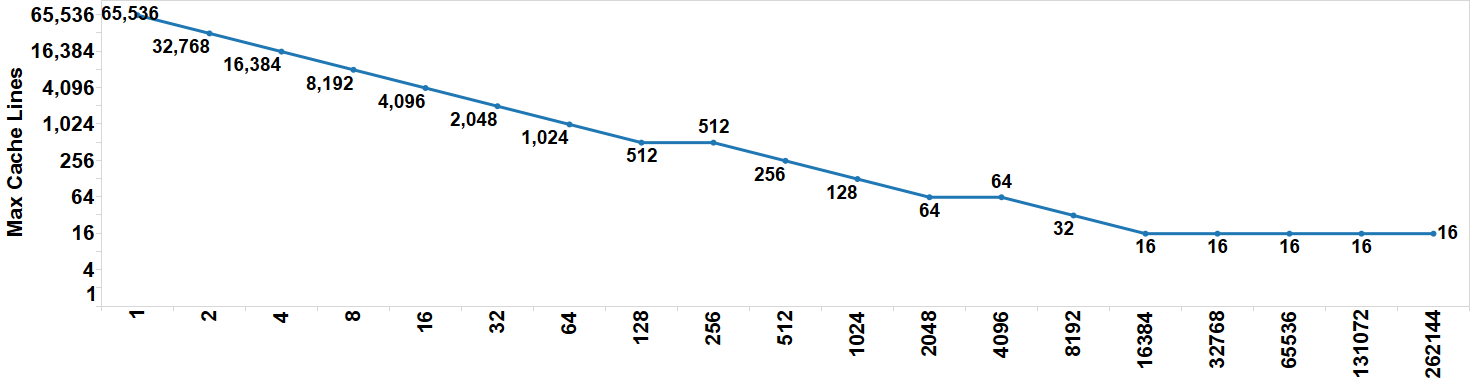
\includegraphics[width=\linewidth]{images/wttm_stride_read_intel}
\caption{Stride Amount vs Cache Lines Readable. Doubling the stride amount halves the size of successful read-only
transactions to a minimum of 16 on the Intel machine}
\label{fig:wttm_stride_read_intel}
\end{figure}


\begin{figure}[H]%[ht!]
\centering
%\figuretitle{Stride Amount vs Cache Lines Writable}
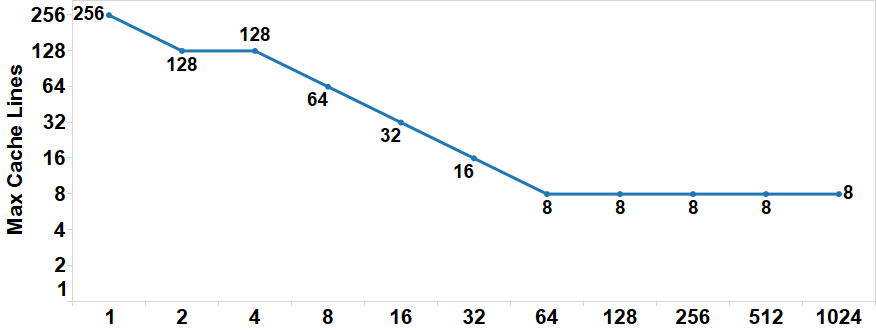
\includegraphics[width=10cm]{images/wttm_stride_write_intel}
\caption{Stride Amount vs Cache Lines Writable. 
Doubling the stride amount halves the size of successful write-only
transactions to a minimum of 8 on the Intel machine}
\label{fig:wttm_stride_write_intel}
\end{figure}


\figref{wttm_capacity_read_intel} summarizes the result of a sequential
read-only access experiment. The data points in the graphs represent the success
probability of the transaction with respect to the number of cache lines read.
The results indicate that a single transaction can reliably read 
around 75,000 contiguous cache lines.

\figref{wttm_stride_read_intel} shows the result of a strided read-only
access experiment. The stride amount is the number of cache lines per
iteration (e.g. reading cache lines 1, 5, 9, 13, 17 etc. 
indicates a stride of 4). Each data point in the graph 
represents the maximum number of cache
lines that can be reliably read with respect 
to the stride amount. For example,
the third data point in the graph indicates 
that when the stride amount is
$2^2$ ($=4$) (e.g. accessing every fourth cache line), 
the transaction can reliably read
$2^{14}$ ($=16,384$) cache lines and commit. 
The significance of this graph is that
the number of cache lines that can be read in a 
single transaction is generally
halved as we double the stride amount, presumably 
because the access pattern
accesses the same few cache sets while 
completely skipping over other sets.
It is important to note that the plot plateaus 
at $2^4$ ($=16$) cache lines, which is not-coincidentally
the associativity of the {L3} cache.

\figreftwo{wttm_capacity_read_intel}{wttm_stride_read_intel} show experimental results that indicate
that the read set is maintained in the
{L3} cache. The {L3} cache of this Intel machine has a maximum
capacity of $2^{17}$ cache lines, which explains 
why read-only transactions
cannot fit much more than $2^{16}$ ($=65,536$) 
cache lines because it is unlikely
for the whole read set to fit perfectly into the {L3} due to
the hash function mapping physical address to L3 cache bank. 
The minimum of 16
cache lines readable when the stride amounts 
are large enough to consecutively
hit the same cache set further supports the notion that the read set is
maintained through the {L3} because this value exactly coincides 
with the L3 associativity.

We also conducted similar experiments for write-only accesses
patterns.  \figref{wttm_capacity_write_intel} illustrates 
the result of an
identical array access experiment, except that the 
transactions are write-only
instead of read-only. A single write-only transaction 
can reliably commit about 400 contiguous cache lines. The
size of the {L1} cache is 512 cache lines and a transaction must also
have sufficient space to store other program metadata (e.g. the
head of the program stack). 

\figref{wttm_stride_write_intel} illustrates that the number of cache
lines that can be written in a single transaction 
is also generally halved as we
double the stride amount, but even as we increase the stride amount
significantly, the number of cache lines that a 
transaction can reliably write
to does not fall below 8, corresponding to the associativity 
of the L1 cache.  This suggests that, at worst, one is limited 
to storing all writes in a single, but entire, set of the L1 cache.

\subheading{IBM}

In this section, we experimentally support the hypothesis
that the IBM HTM implementation uses a dedicated structure
to store read and write sets, choosing not to extend the 
functionality of the existing cache structures as with
the Intel implementation.

The results of our strided access experiment for 
both read-only and write-only
transactions appear to be identical in
\figref{wttm_stride_readwrite_ibm}; the
doubling-stride-amount-halving-transaction-size 
effect is still observed and a
minimum of 16 cache lines can be read or written in a single transaction.

The maximum observed hardware transaction size of 
63 shown in \figref{wttm_capacity_readwrite_ibm} is far too
small to be attributed to even the {L1} cache, which holds 512 cache
lines. The identical measurements between the read and write set 
found in 
\figreftwo{wttm_capacity_readwrite_ibm}{wttm_stride_readwrite_ibm} suggest that there is little distinction
between the handling of reads and writes in a transaction on the IBM machine.
From these results, we conclude that there are dedicated caches for transactions
on the IBM machine and, more generally, for the PowerPC architecture. The
dedicated caches likely each have 4 cache sets and a set associativity of 16,
for a total of 64 cache lines.

\begin{figure}[]%[ht!]
\centering
%\figuretitle{Cache Lines Read/Written vs Success Probability}
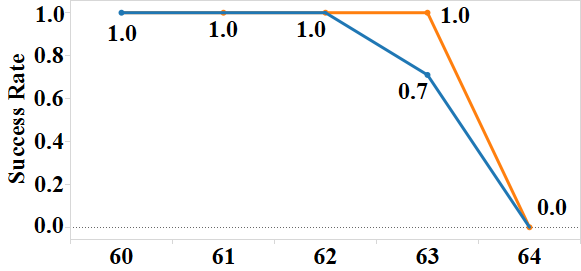
\includegraphics[width=\linewidth]{images/wttm_capacity_readwrite_ibm}
\caption{Cache Lines Read/Written vs Success Probability. 
The read set and write set maximum sequential access capacity on the
IBM machine is 63 cache lines}
\label{fig:wttm_capacity_readwrite_ibm}
\end{figure}

\begin{figure}[]%[ht!]
\centering
%\figuretitle{Stride Amount vs Cache Lines Readable/Writeable}
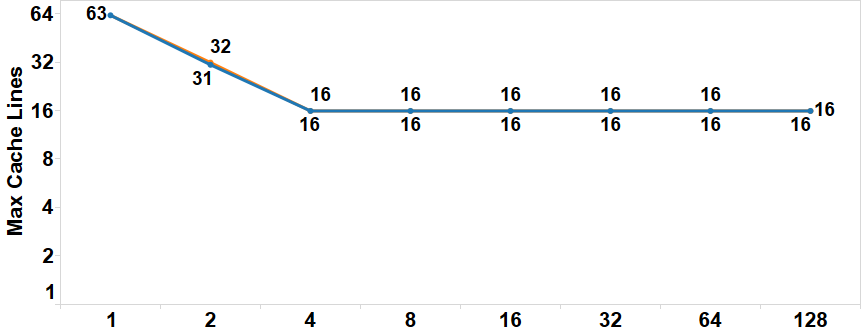
\includegraphics[width=100mm]{images/wttm_stride_readwrite_ibm}
\caption{Stride Amount vs Cache Lines Readable/Writeable. 
Doubling the stride amount halves the size of successful read-only and
write-only transactions to a minimum of 16 on the IBM machine}
\label{fig:wttm_stride_readwrite_ibm}
\end{figure}

\begin{figure}[]%[ht!]
\centering
%\figuretitle{Number of Threads vs Committed Transactions}
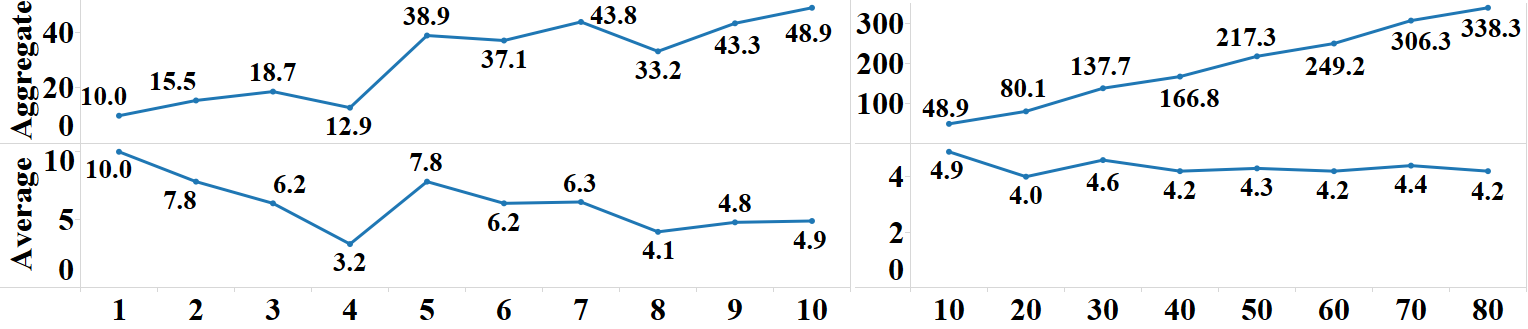
\includegraphics[width=\linewidth]{images/wttm_core_or_thread_ibm}
\caption{Number of Threads vs Committed Transactions. 
Aggregate committed transactions increases with the number of threads
while average committed transactions remains constant, suggesting that there is
a dedicated cache per core on the IBM machine}
\label{fig:wttm_core_or_thread_ibm}
\end{figure}

A natural next question is whether this IBM machine has 10 dedicated caches that
are spread across each core, or if there are 80 dedicated caches that are spread
across each hardware thread. To determine the difference, we experimented and
measured the number of successful write-only transactions that concurrently
running threads were able to complete. Each thread makes 10000 transaction
attempts to write 40 thread-local padded cache lines and then commit. The
transaction size of 40 cache lines is designed to sufficiently fill up the
dedicated caches per transaction to induce capacity aborts in the case of shared
caches.

We see in \figref{wttm_core_or_thread_ibm} compelling reason to believe that
there are 80 dedicated caches, one for each hardware thread. Each spawned
software thread is pinned to a unique hardware thread in round robin fashion
such that the distribution is even across the 10 cores. If all 8 of the
hardware threads on a single core share a single dedicated cache, we would
expect to see sublinear speedup, perhaps even degraded performance, as we spawn
more running threads and assign them to the same core. Instead, we observe a
linear increase in the aggregate number of successfully committed transactions,
while the average per-thread number of successful transactions is constant.
Although the general 45\% success rate suggests some level of contention between
the running threads, it is most likely not due to per-core sharing of a
dedicated cache.
 
